\section{Descripción del prototipo}
El prototipo actual busca que sea posible integrar los datos del caso de estudio a el cluster definido en el prototipo 1 que se encuentra en el capitulo \nameref{cap:Cap3}.
\\
Una vez que los datos sean cargados a los nodos, se busca comprobar que el cluster siga funcionando correctamente y que se puedan hacer consultas sobre los datos que este almacena, comprobando con esto su accesibilidad, disponibilidad y correcta asignación de los mismos a la red.
\section{Análisis}
\subsection{Análisis de la adaptación de los datos a la red distribuida}
%explicar hadoop 
El archivo de datos correspondiente al caso de estudio cuenta con 21GB de texto plano. Debido a que se definió que cada nodo de datos/replica cuenta con al menos 40GB de almacenamiento.Los datos podrán ser almacenados en la red distribuida sin causar problemas de almacenamiento ya que estos son soportados por las capacidades definidas en el prototipo 1 que fueron establecidas contemplando esta condición.
% Los datos correspondientes podrán ser adaptados al ambiente creado sin mayores complicaciones ya que esto es algo que ya se tenia contemplado desde el prototipo 1.
\\
Para poder adaptar los datos del caso de estudio a la red distribuida creada con anterioridad se hará uso de Apache Hadoop. 
\\
Esto debido a que este cuenta con Hadoop Distributed File System (HDFS). HDFS  es  un  sistema  de  archivos  distribuido  y  tolerante  a  fallos. Funciona  sobre  el  
conjunto  de  los  nodos  de  un  cluster  de  Hadoop,  balanceando  la  carga  de  archivos   entre   las   máquinas   del   cluster,   de   forma   equitativa.   Gracias   a   su   
naturaleza  distribuida,  proporciona  alta  disponibilidad  y  altas  prestaciones  que  le  permiten ser capaz de manejar archivos de gran tamaño.
\\
por lo que, haciendo uso de este sistema de manejo de archivos y teniendo las capacidades de almacenamiento en los nodos de la red distribuida es posible afirmar que se puede adaptar sin complicaciones el archivo de datos del caso de estudio.

\section{Diseño}
\subsection{Diseño de la red distribuida con nodos de datos}
La red distribuida cuenta con 3 nodos de datos/replica y un nodo maestro, una vez que se apliquen las configuraciones correspondientes a la asignación de los datos en los nodos de datos/replica así como un algoritmo para probar que los datos asignados son accesibles, la red distribuida deberá verse como la que se muestra en la imagen \nameref{fig:redi3}
\newpage
\begin{figure}[!htbp]
	\hypertarget{fig:redi3}{\hspace{1pt}}
	\begin{center}
		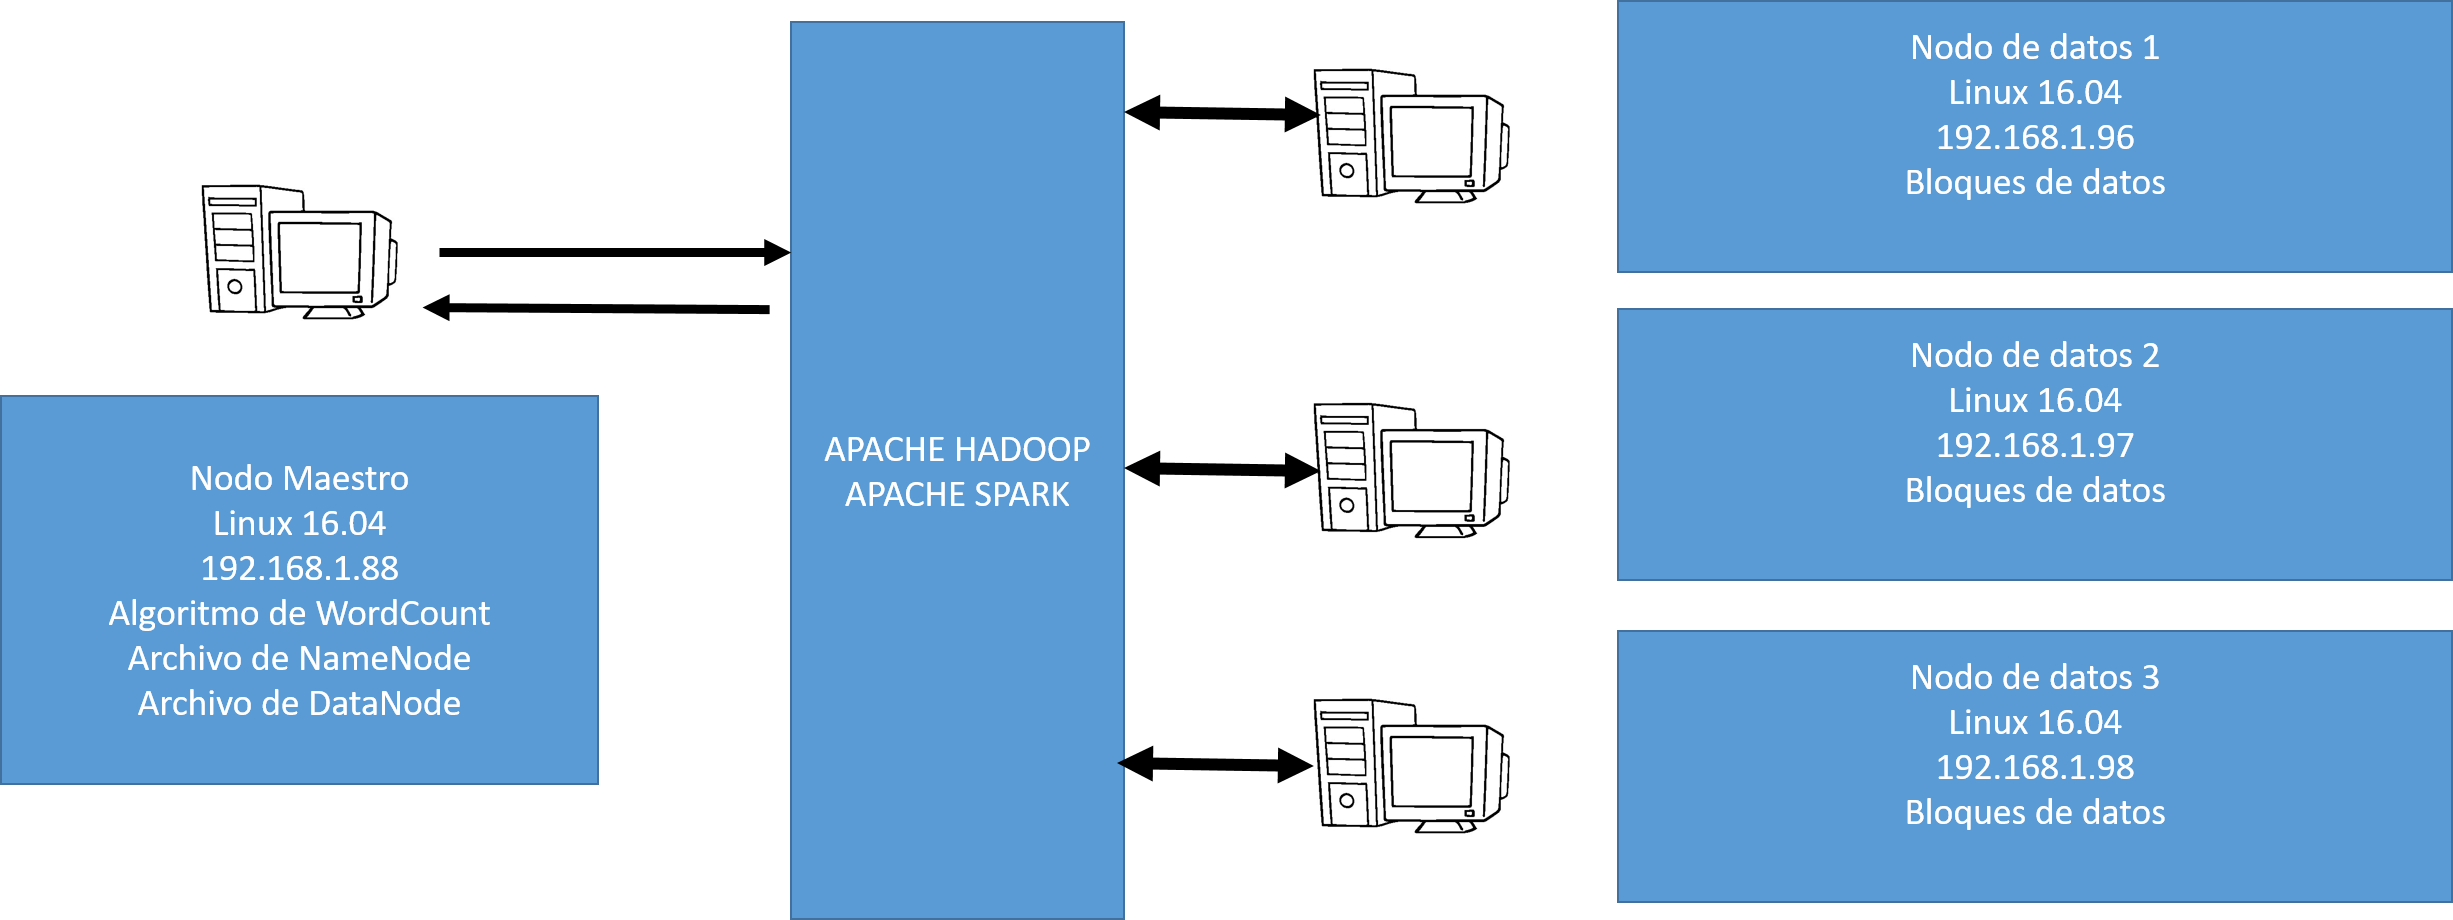
\includegraphics[width=.7\textwidth]{capitulo4/images/im3.png}
		\caption{Diseño de la red distribuida con nodos de datos}
		\label{fig:redi3}
	\end{center}
\end{figure}
la cual funciona conectando el cluster a una red local que les de una IP a cada uno de ellos la cual será definida como estática y se utilizara para las conexiones de manera distribuida tanto de Apache Hadoop como también de Apache Spark. 
\\
Los nodos de datos/replica no se comunicarán entre si al momento de ejecutar operaciones de computo en la red distribuida y para tal motivo utilizarán la conexión con el nodo maestro.
\\
%diagrama de como quedo constituida la red distribuida con apache hadoop y spark 
\subsection{Diseño de pruebas de obtención de información}
\label{osh}
Para poder conocer si los datos fueron distribuidos correctamente y el cluster se encuentra en funcionamiento es posible utilizar un algoritmo que use los datos que se encuentran en el cluster y al final regrese un resultado.
\\
Los algoritmos de big data que serán necesarios para este trabajo son algoritmos que utilizan como base una tecnología llamada Map Reduce.
\\
Se encontró que existen algoritmos de prueba dentro de Hadoop que pueden ser utilizados para comprobar el correcto funcionamiento de la red. sin embargo, se busco comprender como es que estas pruebas funcionan.
\\
Y a su vez buscar que el ejemplo que sea aplicado sobre los datos del caso de estudio se adapte mejor a estos y ofrezca resultados mas interesantes.  
\\
\subsubsection{WordCount tradicional}
La prueba que se va a realizar es el "Contador de palabras" o "WordCount" este algoritmo lo que hace es contar todas las palabras que se encuentran dentro de un archivo y decir cuantas coincidencias de la misma palabra se encontraron. 
\\ 
El algoritmo funciona de la siguiente manera:
\begin{itemize}
\item Cada que encuentra una nueva palabra la agrega al listado de palabras con el valor de 1 que significa que solo ha sido encontrada una vez.
\item En caso de que la palabra sea encontrada nuevamente, entonces se reemplazara el número asociado a esa palabra por el número que tenia en ese momento + 1.
\item Termina cuando llega al final del archivo y por lo tanto todas las palabras nuevas fueron registradas y se conoce cuantas veces aparecen en el archivo.
\end{itemize} 
El procedimiento descrito anteriormente se explicará de igual forma con el diagrama de flujo que se muestra en la Imagen \nameref{fig:redi}.

\begin{figure}[!htbp]
	\hypertarget{fig:redi}{\hspace{1pt}}
	\begin{center}
		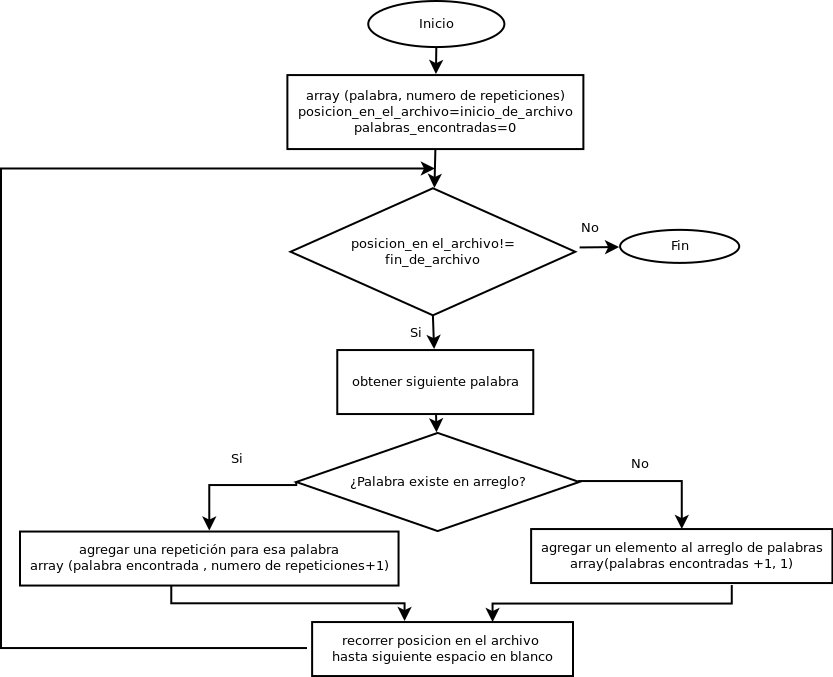
\includegraphics[width=.7\textwidth]{capitulo4/images/im1.png}
		\caption{Diagrama de flujo del algoritmo contador de palabras}
		\label{fig:redi}
	\end{center}
\end{figure}
Los pasos descritos anteriormente, son los pasos que serian utilizados si se tratara de un algoritmo que se ejecuta sin el uso de Map Reduce.
\subsubsection{WordCount con el uso de Map Reduce}
Map Reduce es una técnica que descompone un trabajo grande en tareas individuales las cuales pueden ser ejecutadas por separado en diferentes computadoras que componen un cluster, y estas al final pueden unir sus resultados individuales para calcular los resultados finales.
\\
\label{funcionmap}
\textbf{Función Map}: Toma un conjunto de datos y los convierte en otro conjunto de datos, donde los elementos individuales se dividen en entradas del nuevo conjunto con la estructura (clave-valor).
 \\
de tal forma que lo que una funcion Map en este ejemplo haría seria convertir el conjunto de palabras en un conjunto diferente donde:
Clave: toma el valor de la palabra que se encontró en el archivo
Valor: asigna el valor de 1 a otras las palabras encontradas en el archivo.
Veamos el siguiente conjunto de entrada dentro del archivo:
\begin{lstlisting} 
	botella, refresco, Botella, BOTELLA, Refresco,RefrescO, botellarefresco. 
\end{lstlisting} 
para este archivo el conjunto de salida de la funcion map, seria:
\begin{lstlisting} 
(botella,1), (refresco,1), (Botella,1), (BOTELLA,1),
 (Refresco,1),(RefrescO,1), (botellarefresco,1). 
\end{lstlisting} 
\label{funcionreduce}
\textbf{Función Reduce}: toma la salida del mapa y combina las entradas para generar un conjunto mas pequeño de datos
De tal forma que lo que la función reduce haría en este ejemplo seria buscar las palabras que sean las mismas de las entregadas por cada nodo y agruparlas. 
veamos el mismo ejemplo, suponiendo que el trabajo fue realizado por 3 nodos de datos, veamos lo que haría la función reduce.
\begin{lstlisting} 
nodo1
(botella,1), (refresco,1).
nodo2
(Botella,1), (BOTELLA,1).
nodo3
(Refresco,1),(RefrescO,1), (botellarefresco,1). 
\end{lstlisting} 
para estas entradas, el conjunto de salida de la función reduce seria:
\begin{lstlisting} 
(BOTELLA,3), (REFRESCO,3), (BOTELLAREFRESCO,1).
\end{lstlisting} 
Sin embargo, cabe destacar que el sistema de Hadoop no solo trabaja con las funciones map y reduce, sino que tiene otras funciones internas que el sistema controla.
\\
En la imagen \nameref{fig:redi2} se puede visualizar el funcionamiento completo que tendría que ejecutarse en el cluster para llevar a cabo este algoritmo.
\begin{figure}[!htbp]
	\hypertarget{fig:redi2}{\hspace{1pt}}
	\begin{center}
		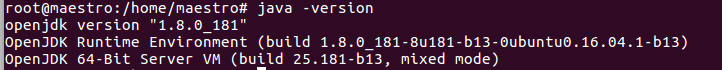
\includegraphics[width=.9\textwidth]{capitulo4/images/im2.png}
		\caption{Funcionamiento completo de Hadoop, con todas sus operaciones}
		\label{fig:redi2}
	\end{center}
\end{figure}
Teniendo como referencia la imagen \nameref{fig:redi2} se explicarán los módulos que ejecuta Hadoop de forma interna para una aplicación Map Reduce de forma breve.
\begin{enumerate}
	\item \textbf{Partición}: Se requiere definir un parametro de partición, esto para que se puedan reconocer las unidades a analizar y con esto poder asignar tareas a los nodos. el parámetro de partición puede ser cualquier cosa, por ejemplo, dividir por espacio, coma, punto y coma, o incluso por una nueva línea ('\ n').
	\item \textbf{Mapeo}: Se explico anteriormente en \nameref{funcionmap} \texttt{Función Map}.
	\item \textbf{Partición intermedia}:Se busca generar grupos con los datos que después de pasar por el modulo de mapeo y tener la estructura de salida de este modulo tienen la misma CLAVE, al cumplir esta condición se asignan en el mismo grupo. Se generan tantos grupos como claves existan.
	\item \textbf{Reducción}: Se explico anteriormente en \nameref{funcionreduce} \texttt{Función Reduce}. 
	\item \textbf{Combinación}: Todos los datos de salida que arrojo la función de reducción son combinados y puestos en un solo grupo para generar un resultado final.
\end{enumerate}

\section{Desarrollo}
Para que Instalar Apache Hadoop en la red distribuida en funcionamiento se siguió el Manual de Instalación de Luminus 
en sus secciones 
\begin{verbatim}
4. Instalación de Apache Hadoop en el nodo maestro
	4.1. Instalación de Hadoop 
		4.1.1. Configuración
		4.1.2. Archivos de configuración
5. Instalación de Apache Hadoop en los nodos de datos
	5.1. Instalación de Hadoop en los nodos de datos 
		5.1.1. Configuración 
6. Puesta en funcionamiento
	6.1. Puesta en funcionamiento del Cluster manejado por el Servidor Apache Hadoop
\end{verbatim}
Las cuales nos permitirán instalar Apache Hadoop el cual tendrá al mismo tiempo todas las configuraciones necesarias
requeridas para este proyecto, tanto en el nodo maestro como también en los nodos de datos/replica.
Dentro del manual de instalación se explica para cada uno de los archivos de configuración de hadoop como es que
estos se configuran y cual es el objetivo de cada configuración de manera detallada.
Una vez que las configuraciones se hayan ejecutado de manera correcta y el cluster se encuentre en funcionamiento
haciendo uso de hadoop, se subirá un archivo a la plataforma, esto se hará siguiendo el manual de instalación de luminus
en la sección
\begin{verbatim}
6.2. Subir un archivo al HDFS
\end{verbatim}
En el momento de subir el archivo al HDFS se puede comprobar que la red distribuida permite realizar esta operación
para lo cual es indispensable comunicarse con todos los nodos que se encuentran dentro de la misma. Esto con el
objetivo de realizar el almacenamiento de manera distribuida haciendo uso de todos los nodos de datos/replica. Por lo
tanto se sabe que la red distribuida tiene conectividad y se encuentra funcionando de manera apropiada.
\subsection{Algoritmo de prueba}
El siguiente algoritmo escrito en JAVA servirá para comprobar que se pueden realizar operaciones sobre los datos
que se encuentran en el cluster.
\\
Como se explico en la sección \nameref{osh} de este capitulo, se utilizará el algoritmo wordcount para cumplir con este objetivo.
También, se menciono que las únicas secciones que se requiere programar para ejecutar un algoritmo de tipo map
reduce es la función map y la función reduce. ya que hadoop se encarga de el resto de funciones.
\\
Por otro lado se explico la forma en que este algoritmo en particular funcionar y un ejemplo de su funcionamiento en
la imagen \nameref{fig:redi2}.
\\
Se decidió que se considere que se encontró una palabra cada que aparezca una ","dentro del archivo como parámetro
de la función de partición, esto debido a que cada atributo de la tabla de datos esta separado por una coma y esto nos
permitiría comprobar cuantas veces aparece un atributo dentro del archivo en lugar de solamente conocer la repetición
de las palabras por separado. Lo cual esta orientado para el archivo de datos del caso de estudio y nos puede dar
información de la frecuencia con la que ciertos registros aparecen dentro del mismo.
\\
El codigo JAVA para tal objetivo se puede visualizar en el \nameref{anexoa}
dentro del cual se pueden destacar algunas observaciones
\begin{itemize}
	\item Se importan las librerías de Apache Hadoop para que pueda reconocerse que se trata de un programa Map Reduce
	que se ejecutará sobre este programa.
	\item Se tiene la clase main la cual principalmente manda a llamar a las clases map y reduce,establece los valores por
	defecto para empezar a contar, Establece los canales de lectura y escritura para que este pueda acceder a los
	archivos del cluster a analizar y pueda tambien escribir sus resultados.
	\item Se tiene la clase map la cual toma la palabra encontrada y le da la estructura (CLAVE, VALOR) , además de
	pasarla a mayúsculas para que considere que se trata de la misma palabra cuando tenga las mismas letras sin
	importar si originalmente estaba escrita en mayúsculas, minúsculas o una combinación de ambas.
	\item La clase reduce que cuenta cuantas veces se repiten en total las palabras en el grupo que se genero de todas las
	palabras iguales que se encontraron en cada uno de los nodos. para sacar una suma total para cada palabra del
	archivo.
\end{itemize}
Este algoritmo tiene que ser compilado ya sea con un IDE de java o directamente desde Hadoop para generar el jar
que posteriormente sera ejecutado por Hadoop.
\\
El codigo desde consola para generar este JAR es el siguiente.
\\
\begin{verbatim}
	bin/hadoop com.sun.tools.javac.Main [clase_principal_java].java
	jar cf [Nombre_jar].jar [clase_principal_java]*.class
\end{verbatim}
\section{Pruebas}
Una vez que se tiene el .JAR a ejecutar se puede hacer uso del siguiente comando para que este entre en funcionamiento dentro de la red distribuida.
\\
\begin{verbatim}
	yarn jar <ruta/a/archivo.jar> <NombreDeClase> <Parametros>
\end{verbatim}
Para nuestro ejemplo especifico el comando seria:
\begin{verbatim}
root@maestro:/opt/hadoop/etc/hadoop: yarn jar /home/mayra/Escritorio/MRProgramsDemo.jar 
PackageDemo.WordCount "user/root/productos/inserts.txt" output6
\end{verbatim}
output6 sera una carpeta que se creará en el sistema de archivos de HDFS para almacenar los resultados de salida.
Esta carpeta puede tener el nombre que se desee y se asigna en esta sección, sin embargo, no puede existir dentro del
sistema de archivos al momento de ejecutar este comando. La carpeta se creará en el directorio /user/root/nombreasignado
\\
Una vez que se ejecute esta instrucción se procederá a revisar las conexiones con los nodos y hacer los ajustes necesarios
para comenzar a ejecutar este algoritmo.
esta información de salida y el comienzo de la ejecución del algoritmo con la parte de la función map pueden verse en
la imagen \nameref{fig:redi4}
este algoritmo.
\begin{figure}[!htbp]
	\hypertarget{fig:redi4}{\hspace{1pt}}
	\begin{center}
		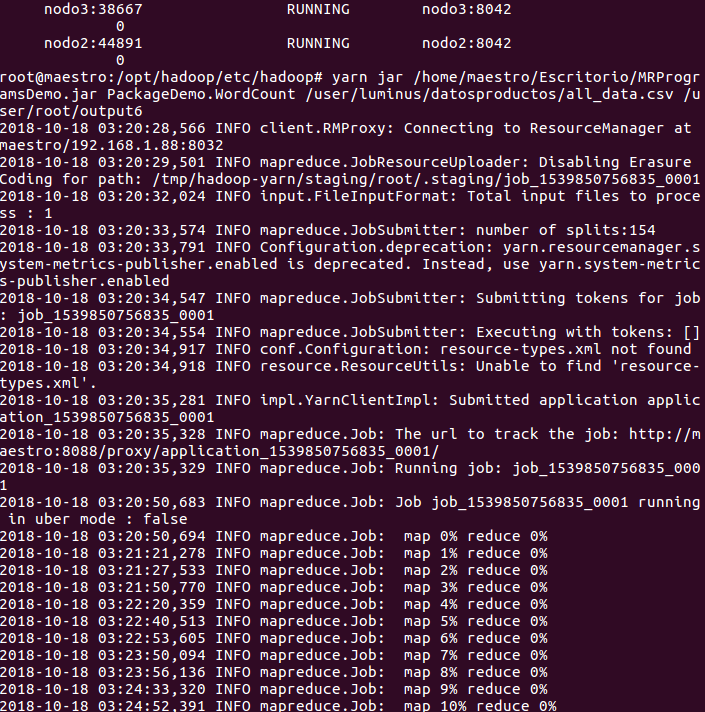
\includegraphics[width=.9\textwidth]{capitulo4/images/ejemplo2.png}
		\caption{Ejecución de algoritmo map reduce para contar palabras: Comenzando el proceso}
		\label{fig:redi4}
	\end{center}
\end{figure}
esto se hará para todos los porcentajes de la función map, una vez que estos finalicen, comenzará a ejecutar
la función reduce y con ella sus porcentajes de progreso como se muestra en la imagen \nameref{fig:redi5}.
\begin{figure}[!htbp]
	\hypertarget{fig:redi5}{\hspace{1pt}}
	\begin{center}
		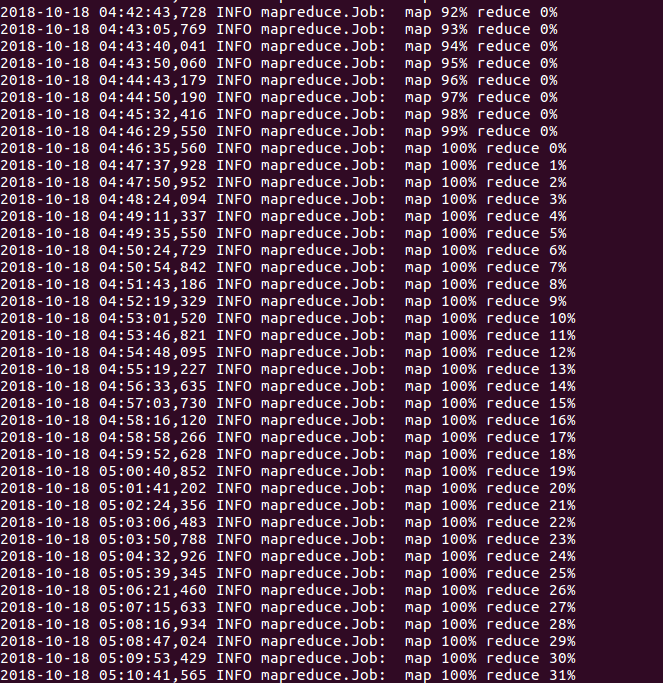
\includegraphics[width=.9\textwidth]{capitulo4/images/ejemplo3.png}
		\caption{Ejecución de algoritmo map reduce para contar palabras: Inicio de funcion reduce}
		\label{fig:redi5}
	\end{center}
\end{figure}
\newpage
Cuando se complete la función reduce procederá a notificar que el algoritmo fue ejecutado correctamente y mostrará
estadísticas de:
\begin{itemize}
	\item File System Counter
	\item Job Counter
	\item MapReduce Framework
\end{itemize}
Dichas estadisticas y resultados finales para este algoritmo se muestran en las figuras \nameref{fig:redi6} y \nameref{fig:redi7}
\begin{figure}[!htbp]
	\hypertarget{fig:redi6}{\hspace{1pt}}
	\begin{center}
		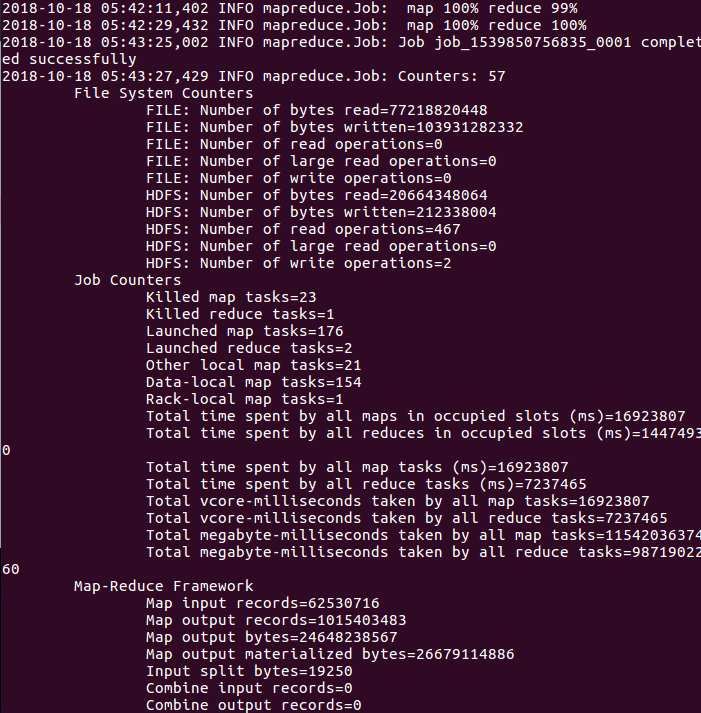
\includegraphics[width=.9\textwidth]{capitulo4/images/ejemplo6.png}
		\caption{Ejecución de algoritmo map reduce para contar palabras: Termina la ejecución del algoritmo}
		\label{fig:redi6}
	\end{center}
\end{figure}
\newpage
\begin{figure}[!htbp]
	\hypertarget{fig:redi7}{\hspace{1pt}}
	\begin{center}
		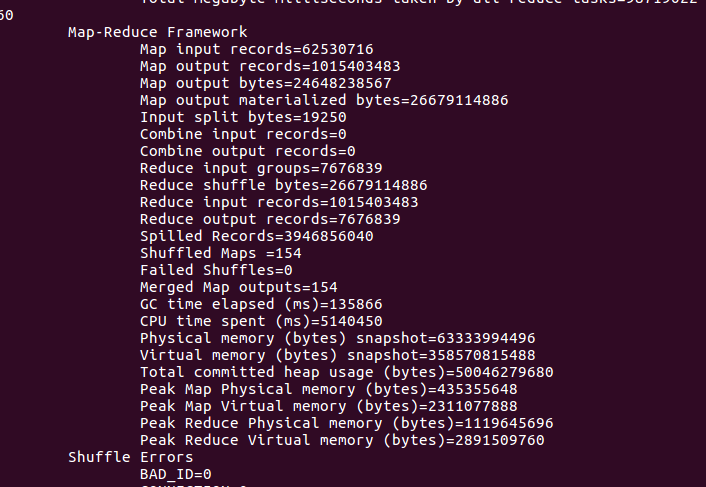
\includegraphics[width=.9\textwidth]{capitulo4/images/ejemplo8.png}
		\caption{Ejecución de algoritmo map reduce para contar palabras: Estadísticas}
		\label{fig:redi7}
	\end{center}
\end{figure}
Ahora, para poder visualizar el resultado de este algoritmo se puede hacer un listado de los archivos que contiene el directorio de salida
que se creo, para ello se utiliza el comando siguiente
\begin{verbatim}
root@maestro:/opt/hadoop/etc/hadoop:hdfs dfs -ls /user/root/output6
\end{verbatim}
Con lo cual se genera la salida que se despliega en la imagen \ref{fig:redi8} la cual muestra que la operación fue exitosa y las dimensiones generadas para el archivo de salida.
\begin{figure}[!htbp]
	\hypertarget{fig:redi8}{\hspace{1pt}}
	\begin{center}
		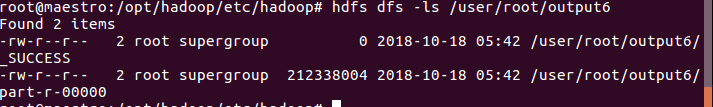
\includegraphics[width=.9\textwidth]{capitulo4/images/ejemplo9.png}
		\caption{Contenido del directorio de salida}
		\label{fig:redi8}
	\end{center}
\end{figure}

Debido a que se trata de un archivo muy grande, para efectos de simplificación solo se mostrará en este documento un
fragmento de dicho archivo que deje ver el trabajo que fue realizado dicho fragmento se muestra en la imagen \ref{fig:redi9}.
\begin{figure}[!htbp]
	\hypertarget{fig:redi9}{\hspace{1pt}}
	\begin{center}
		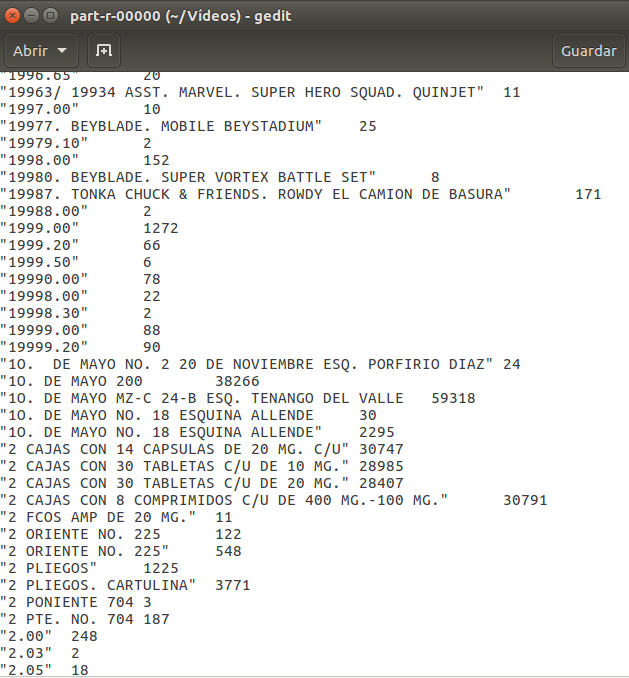
\includegraphics[width=.9\textwidth]{capitulo4/images/ejemplo10.png}
		\caption{Contenido del archivo de resultados}
		\label{fig:redi9}
	\end{center}
\end{figure}
Dentro de esta imagen podemos ver por ejemplo, cuantas veces aparecen determinados precios dentro del archivo,
direcciones o bien descripciones de productos, entre otros.\\
Por lo cual se puede ver que el archivo fue estudiado en su totalidad y que se tienen coincidencias para diferentes
entradas que se encontraban dentro del archivo.\\
Un resultado interesante obtenido que se puede observar en la imagen \ref{fig:redi10} es que, al menos para este archivo la fecha
de registro es irrelevante pues para cada articulo se tiene una diferente o bien comparten una misma fecha cuando la
hora establecida es 0hrs para una gran cantidad de registros que fueron dados de alta el mismo día, pero en realidad
no proporciona información real de los articulos y genera mucho ruido en el archivo.\\
Existen mas entradas de fechas que información de los productos, comportamiento que dificultaría el análisis de los
datos en un futuro por lo cual este atributo sera retirado del archivo correspondiente al caso de estudio.
\begin{figure}[!htbp]
	\hypertarget{fig:redi9}{\hspace{1pt}}
	\begin{center}
		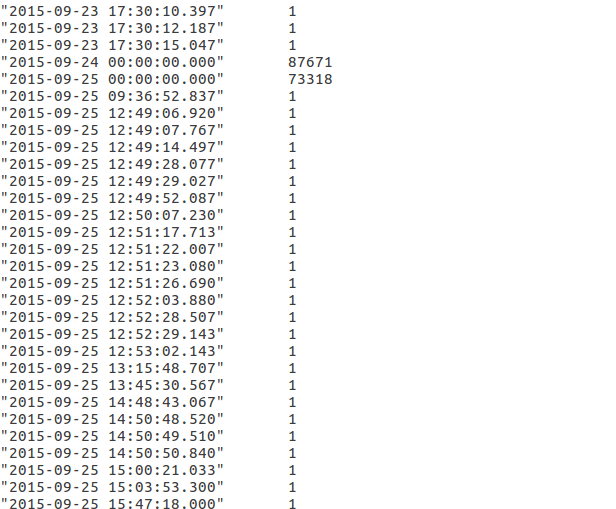
\includegraphics[width=.9\textwidth]{capitulo4/images/ejemplo11.png}
		\caption{Fechas de registro en el archivo de resultados}
		\label{fig:redi10}
	\end{center}
\end{figure}
Con lo que podemos concluir:
\begin{itemize}
	\item El cluster funciona correctamente
	\item Existe comunicación entre los nodos
	\item Los nodos de datos/replica son capaces de identificar al nodo maestro y recibir instrucciones de el
	\item El nodo maestro es capaz de comunicar trabajos a los nodos de datos/replica y de interpretar los resultados de
	sus trabajos de manera satisfactoria
	\item Se tiene el archivo del caso de estudio almacenado de manera distribuida en los nodos
	\item El archivo del caso de estudio es accesible y se pueden ejecutar operaciones sobre de el
\end{itemize}
Por lo tanto, el prototipo dos concluye de manera exitosa